\documentclass[12pt]{article}

\usepackage{amsfonts}
\usepackage{enumitem}
\usepackage{graphicx}

\begin{document}
\thispagestyle{empty}
\begin{center}
\Large{\textbf{ECON 634 Problem Set 2}}\\[3mm]
\large{{Mingyang Li}}\\[1mm]
\today
\end{center}

\begin{enumerate}
\item The functional equation of the dynamic programming problem is
$$V(k)=\max_{k'} \left\{\frac{[A^hk^\alpha+(1-\delta)k-k']^{(1-\sigma)}}{1-\sigma}+\beta\mathbb{E}V(k')\right\}$$
where $k$ is the state variable and $k'$ is the control variable.
\item Yes, according to the plot of the value function over $K$, it is concave and increasing in $K$.
\begin{center}
  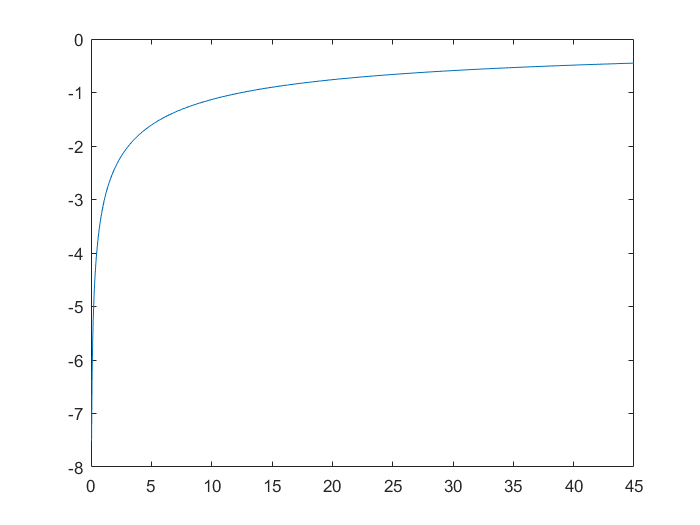
\includegraphics[width=63.5mm]{VKstochastic.png}
\end{center}
\item Yes, according to the plot of the policy function over $K$, it is concave and increasing in $K$.
\begin{center}
  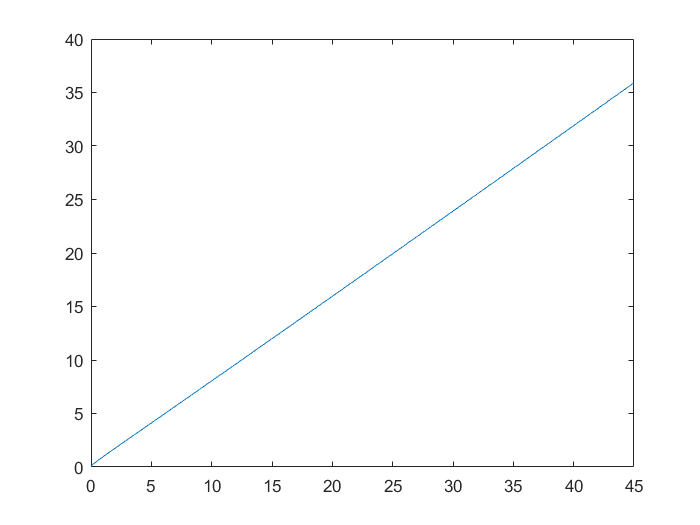
\includegraphics[width=63.5mm]{GKstochastic.png}
\end{center}
\end{enumerate}

\end{document}